

\tikzset{every picture/.style={line width=0.75pt}} %set default line width to 0.75pt        

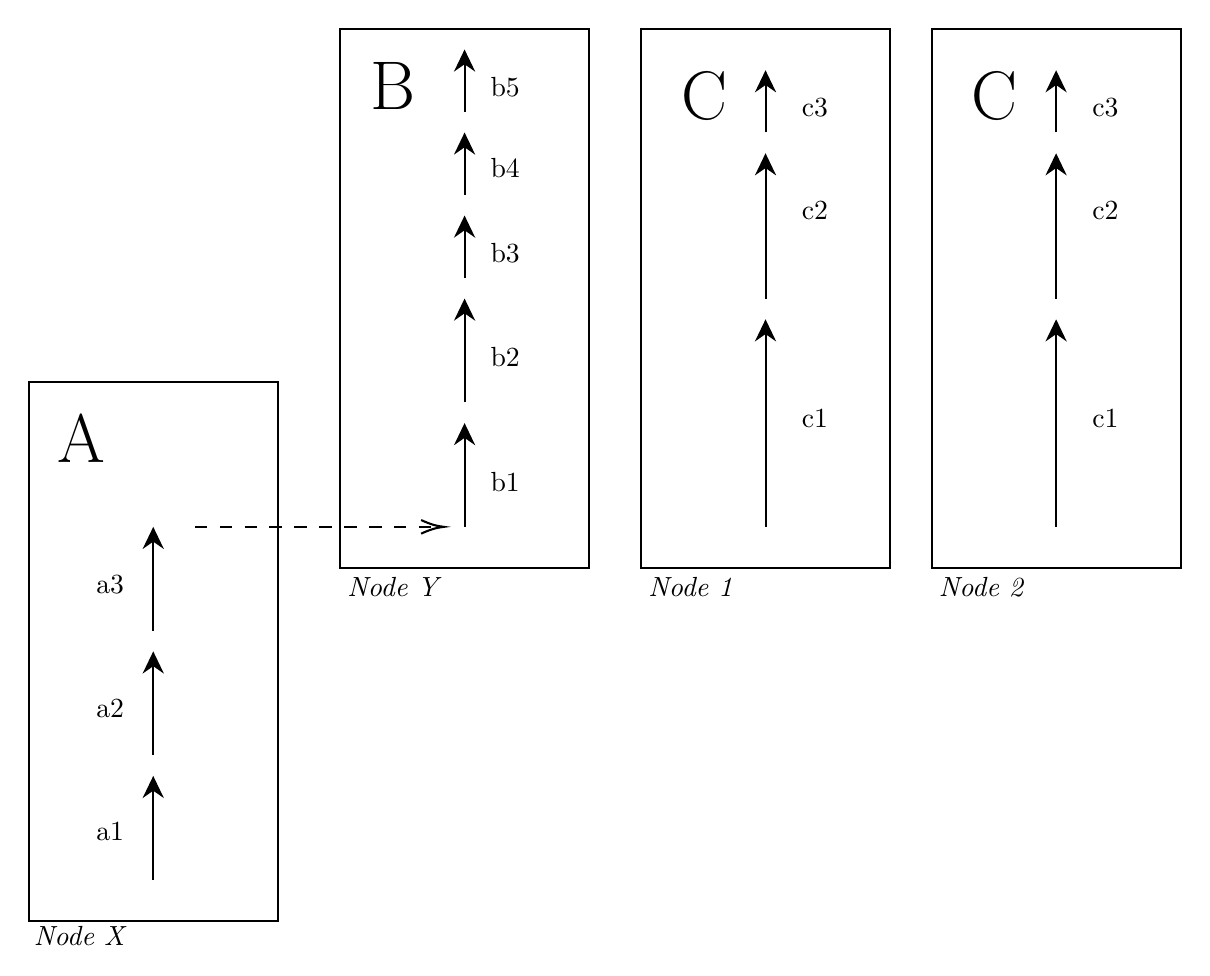
\begin{tikzpicture}[x=0.75pt,y=0.75pt,yscale=-1,xscale=1]
%uncomment if require: \path (0,463); %set diagram left start at 0, and has height of 463

%Straight Lines [id:da27430706126077264] 
\draw [color={rgb, 255:red, 0; green, 0; blue, 0 }  ,draw opacity=1 ][fill={rgb, 255:red, 255; green, 0; blue, 0 }  ,fill opacity=1 ][line width=0.75]    (80,420) -- (80,373) ;
\draw [shift={(80,370)}, rotate = 450] [fill={rgb, 255:red, 0; green, 0; blue, 0 }  ,fill opacity=1 ][line width=0.08]  [draw opacity=0] (10.72,-5.15) -- (0,0) -- (10.72,5.15) -- (7.12,0) -- cycle    ;
%Straight Lines [id:da18541775456344745] 
\draw [color={rgb, 255:red, 0; green, 0; blue, 0 }  ,draw opacity=1 ][fill={rgb, 255:red, 144; green, 19; blue, 254 }  ,fill opacity=1 ][line width=0.75]    (80,360) -- (80,313) ;
\draw [shift={(80,310)}, rotate = 450] [fill={rgb, 255:red, 0; green, 0; blue, 0 }  ,fill opacity=1 ][line width=0.08]  [draw opacity=0] (10.72,-5.15) -- (0,0) -- (10.72,5.15) -- (7.12,0) -- cycle    ;
%Straight Lines [id:da9191051295157292] 
\draw    (80,300) -- (80,253) ;
\draw [shift={(80,250)}, rotate = 450] [fill={rgb, 255:red, 0; green, 0; blue, 0 }  ][line width=0.08]  [draw opacity=0] (10.72,-5.15) -- (0,0) -- (10.72,5.15) -- (7.12,0) -- cycle    ;
%Straight Lines [id:da565354971469586] 
\draw [color={rgb, 255:red, 0; green, 0; blue, 0 }  ,draw opacity=1 ][line width=0.75]    (230,250) -- (230,203) ;
\draw [shift={(230,200)}, rotate = 450] [fill={rgb, 255:red, 0; green, 0; blue, 0 }  ,fill opacity=1 ][line width=0.08]  [draw opacity=0] (10.72,-5.15) -- (0,0) -- (10.72,5.15) -- (7.12,0) -- cycle    ;
%Straight Lines [id:da6700429327448342] 
\draw [color={rgb, 255:red, 0; green, 0; blue, 0 }  ,draw opacity=1 ][line width=0.75]    (230,190) -- (230,143) ;
\draw [shift={(230,140)}, rotate = 450] [fill={rgb, 255:red, 0; green, 0; blue, 0 }  ,fill opacity=1 ][line width=0.08]  [draw opacity=0] (10.72,-5.15) -- (0,0) -- (10.72,5.15) -- (7.12,0) -- cycle    ;
%Straight Lines [id:da28075371980457553] 
\draw [color={rgb, 255:red, 0; green, 0; blue, 0 }  ,draw opacity=1 ]   (230,130) -- (230,103) ;
\draw [shift={(230,100)}, rotate = 450] [fill={rgb, 255:red, 0; green, 0; blue, 0 }  ,fill opacity=1 ][line width=0.08]  [draw opacity=0] (10.72,-5.15) -- (0,0) -- (10.72,5.15) -- (7.12,0) -- cycle    ;
%Straight Lines [id:da9441221295165446] 
\draw [color={rgb, 255:red, 0; green, 0; blue, 0 }  ,draw opacity=1 ]   (230,90) -- (230,63) ;
\draw [shift={(230,60)}, rotate = 450] [fill={rgb, 255:red, 0; green, 0; blue, 0 }  ,fill opacity=1 ][line width=0.08]  [draw opacity=0] (10.72,-5.15) -- (0,0) -- (10.72,5.15) -- (7.12,0) -- cycle    ;
%Straight Lines [id:da3794379224544834] 
\draw [color={rgb, 255:red, 0; green, 0; blue, 0 }  ,draw opacity=1 ][line width=0.75]    (230,50) -- (230,23) ;
\draw [shift={(230,20)}, rotate = 450] [fill={rgb, 255:red, 0; green, 0; blue, 0 }  ,fill opacity=1 ][line width=0.08]  [draw opacity=0] (10.72,-5.15) -- (0,0) -- (10.72,5.15) -- (7.12,0) -- cycle    ;
%Straight Lines [id:da13857817807873274] 
\draw [color={rgb, 255:red, 0; green, 0; blue, 0 }  ,draw opacity=1 ]   (375,250) -- (375,153) ;
\draw [shift={(375,150)}, rotate = 450] [fill={rgb, 255:red, 0; green, 0; blue, 0 }  ,fill opacity=1 ][line width=0.08]  [draw opacity=0] (10.72,-5.15) -- (0,0) -- (10.72,5.15) -- (7.12,0) -- cycle    ;
%Straight Lines [id:da18881367347259226] 
\draw [color={rgb, 255:red, 0; green, 0; blue, 0 }  ,draw opacity=1 ]   (375,140) -- (375,73) ;
\draw [shift={(375,70)}, rotate = 450] [fill={rgb, 255:red, 0; green, 0; blue, 0 }  ,fill opacity=1 ][line width=0.08]  [draw opacity=0] (10.72,-5.15) -- (0,0) -- (10.72,5.15) -- (7.12,0) -- cycle    ;
%Straight Lines [id:da5578630098708864] 
\draw [color={rgb, 255:red, 0; green, 0; blue, 0 }  ,draw opacity=1 ][line width=0.75]    (375,60) -- (375,33) ;
\draw [shift={(375,30)}, rotate = 450] [fill={rgb, 255:red, 0; green, 0; blue, 0 }  ,fill opacity=1 ][line width=0.08]  [draw opacity=0] (10.72,-5.15) -- (0,0) -- (10.72,5.15) -- (7.12,0) -- cycle    ;
%Straight Lines [id:da8425704792181163] 
\draw [color={rgb, 255:red, 0; green, 0; blue, 0 }  ,draw opacity=1 ]   (515,250) -- (515,153) ;
\draw [shift={(515,150)}, rotate = 450] [fill={rgb, 255:red, 0; green, 0; blue, 0 }  ,fill opacity=1 ][line width=0.08]  [draw opacity=0] (10.72,-5.15) -- (0,0) -- (10.72,5.15) -- (7.12,0) -- cycle    ;
%Straight Lines [id:da4623771258590563] 
\draw [color={rgb, 255:red, 0; green, 0; blue, 0 }  ,draw opacity=1 ]   (515,140) -- (515,73) ;
\draw [shift={(515,70)}, rotate = 450] [fill={rgb, 255:red, 0; green, 0; blue, 0 }  ,fill opacity=1 ][line width=0.08]  [draw opacity=0] (10.72,-5.15) -- (0,0) -- (10.72,5.15) -- (7.12,0) -- cycle    ;
%Straight Lines [id:da01593649548581877] 
\draw [color={rgb, 255:red, 0; green, 0; blue, 0 }  ,draw opacity=1 ][line width=0.75]    (515,60) -- (515,33) ;
\draw [shift={(515,30)}, rotate = 450] [fill={rgb, 255:red, 0; green, 0; blue, 0 }  ,fill opacity=1 ][line width=0.08]  [draw opacity=0] (10.72,-5.15) -- (0,0) -- (10.72,5.15) -- (7.12,0) -- cycle    ;
%Shape: Rectangle [id:dp2885118599122133] 
\draw   (20,180) -- (140,180) -- (140,440) -- (20,440) -- cycle ;
%Shape: Rectangle [id:dp29749503322267146] 
\draw   (170,10) -- (290,10) -- (290,270) -- (170,270) -- cycle ;
%Shape: Rectangle [id:dp633340374583701] 
\draw   (315,10) -- (435,10) -- (435,270) -- (315,270) -- cycle ;
%Shape: Rectangle [id:dp5609698959879448] 
\draw   (455,10) -- (575,10) -- (575,270) -- (455,270) -- cycle ;
%Straight Lines [id:da5768510833378265] 
\draw  [dash pattern={on 4.5pt off 4.5pt}]  (100,250) -- (218,250) ;
\draw [shift={(220,250)}, rotate = 180] [color={rgb, 255:red, 0; green, 0; blue, 0 }  ][line width=0.75]    (10.93,-3.29) .. controls (6.95,-1.4) and (3.31,-0.3) .. (0,0) .. controls (3.31,0.3) and (6.95,1.4) .. (10.93,3.29)   ;

% Text Node
\draw (45.5,207.5) node  [font=\Huge] [align=left] {A};
% Text Node
\draw (195.5,37.5) node  [font=\Huge] [align=left] {B};
% Text Node
\draw (345.5,42.5) node  [font=\Huge] [align=left] {C};
% Text Node
\draw (485.5,42.5) node  [font=\Huge] [align=left] {C};
% Text Node
\draw (51,391) node [anchor=north west][inner sep=0.75pt]   [align=left] {a1};
% Text Node
\draw (51,332) node [anchor=north west][inner sep=0.75pt]   [align=left] {a2};
% Text Node
\draw (51,272) node [anchor=north west][inner sep=0.75pt]   [align=left] {a3};
% Text Node
\draw (241,222) node [anchor=north west][inner sep=0.75pt]   [align=left] {b1};
% Text Node
\draw (241,162) node [anchor=north west][inner sep=0.75pt]   [align=left] {b2};
% Text Node
\draw (241,112) node [anchor=north west][inner sep=0.75pt]   [align=left] {b3};
% Text Node
\draw (241,71) node [anchor=north west][inner sep=0.75pt]   [align=left] {b4};
% Text Node
\draw (241,32) node [anchor=north west][inner sep=0.75pt]   [align=left] {b5};
% Text Node
\draw (391,192) node [anchor=north west][inner sep=0.75pt]   [align=left] {c1};
% Text Node
\draw (391,92) node [anchor=north west][inner sep=0.75pt]   [align=left] {c2};
% Text Node
\draw (391,42) node [anchor=north west][inner sep=0.75pt]   [align=left] {c3};
% Text Node
\draw (531,192) node [anchor=north west][inner sep=0.75pt]   [align=left] {c1};
% Text Node
\draw (531,92) node [anchor=north west][inner sep=0.75pt]   [align=left] {c2};
% Text Node
\draw (531,42) node [anchor=north west][inner sep=0.75pt]   [align=left] {c3};
% Text Node
\draw (317,273) node [anchor=north west][inner sep=0.75pt]   [align=left] {\textit{Node 1}};
% Text Node
\draw (457,273) node [anchor=north west][inner sep=0.75pt]   [align=left] {\textit{Node 2}};
% Text Node
\draw (172,273) node [anchor=north west][inner sep=0.75pt]   [align=left] {\textit{Node Y}};
% Text Node
\draw (21,441) node [anchor=north west][inner sep=0.75pt]   [align=left] {\textit{Node X}};


\end{tikzpicture}
